% Options for packages loaded elsewhere
\PassOptionsToPackage{unicode}{hyperref}
\PassOptionsToPackage{hyphens}{url}
\PassOptionsToPackage{dvipsnames,svgnames,x11names}{xcolor}
%
\documentclass[
  letterpaper,
  DIV=11,
  numbers=noendperiod]{scrreprt}

\usepackage{amsmath,amssymb}
\usepackage{iftex}
\ifPDFTeX
  \usepackage[T1]{fontenc}
  \usepackage[utf8]{inputenc}
  \usepackage{textcomp} % provide euro and other symbols
\else % if luatex or xetex
  \usepackage{unicode-math}
  \defaultfontfeatures{Scale=MatchLowercase}
  \defaultfontfeatures[\rmfamily]{Ligatures=TeX,Scale=1}
\fi
\usepackage{lmodern}
\ifPDFTeX\else  
    % xetex/luatex font selection
\fi
% Use upquote if available, for straight quotes in verbatim environments
\IfFileExists{upquote.sty}{\usepackage{upquote}}{}
\IfFileExists{microtype.sty}{% use microtype if available
  \usepackage[]{microtype}
  \UseMicrotypeSet[protrusion]{basicmath} % disable protrusion for tt fonts
}{}
\makeatletter
\@ifundefined{KOMAClassName}{% if non-KOMA class
  \IfFileExists{parskip.sty}{%
    \usepackage{parskip}
  }{% else
    \setlength{\parindent}{0pt}
    \setlength{\parskip}{6pt plus 2pt minus 1pt}}
}{% if KOMA class
  \KOMAoptions{parskip=half}}
\makeatother
\usepackage{xcolor}
\setlength{\emergencystretch}{3em} % prevent overfull lines
\setcounter{secnumdepth}{5}
% Make \paragraph and \subparagraph free-standing
\ifx\paragraph\undefined\else
  \let\oldparagraph\paragraph
  \renewcommand{\paragraph}[1]{\oldparagraph{#1}\mbox{}}
\fi
\ifx\subparagraph\undefined\else
  \let\oldsubparagraph\subparagraph
  \renewcommand{\subparagraph}[1]{\oldsubparagraph{#1}\mbox{}}
\fi

\usepackage{color}
\usepackage{fancyvrb}
\newcommand{\VerbBar}{|}
\newcommand{\VERB}{\Verb[commandchars=\\\{\}]}
\DefineVerbatimEnvironment{Highlighting}{Verbatim}{commandchars=\\\{\}}
% Add ',fontsize=\small' for more characters per line
\usepackage{framed}
\definecolor{shadecolor}{RGB}{241,243,245}
\newenvironment{Shaded}{\begin{snugshade}}{\end{snugshade}}
\newcommand{\AlertTok}[1]{\textcolor[rgb]{0.68,0.00,0.00}{#1}}
\newcommand{\AnnotationTok}[1]{\textcolor[rgb]{0.37,0.37,0.37}{#1}}
\newcommand{\AttributeTok}[1]{\textcolor[rgb]{0.40,0.45,0.13}{#1}}
\newcommand{\BaseNTok}[1]{\textcolor[rgb]{0.68,0.00,0.00}{#1}}
\newcommand{\BuiltInTok}[1]{\textcolor[rgb]{0.00,0.23,0.31}{#1}}
\newcommand{\CharTok}[1]{\textcolor[rgb]{0.13,0.47,0.30}{#1}}
\newcommand{\CommentTok}[1]{\textcolor[rgb]{0.37,0.37,0.37}{#1}}
\newcommand{\CommentVarTok}[1]{\textcolor[rgb]{0.37,0.37,0.37}{\textit{#1}}}
\newcommand{\ConstantTok}[1]{\textcolor[rgb]{0.56,0.35,0.01}{#1}}
\newcommand{\ControlFlowTok}[1]{\textcolor[rgb]{0.00,0.23,0.31}{#1}}
\newcommand{\DataTypeTok}[1]{\textcolor[rgb]{0.68,0.00,0.00}{#1}}
\newcommand{\DecValTok}[1]{\textcolor[rgb]{0.68,0.00,0.00}{#1}}
\newcommand{\DocumentationTok}[1]{\textcolor[rgb]{0.37,0.37,0.37}{\textit{#1}}}
\newcommand{\ErrorTok}[1]{\textcolor[rgb]{0.68,0.00,0.00}{#1}}
\newcommand{\ExtensionTok}[1]{\textcolor[rgb]{0.00,0.23,0.31}{#1}}
\newcommand{\FloatTok}[1]{\textcolor[rgb]{0.68,0.00,0.00}{#1}}
\newcommand{\FunctionTok}[1]{\textcolor[rgb]{0.28,0.35,0.67}{#1}}
\newcommand{\ImportTok}[1]{\textcolor[rgb]{0.00,0.46,0.62}{#1}}
\newcommand{\InformationTok}[1]{\textcolor[rgb]{0.37,0.37,0.37}{#1}}
\newcommand{\KeywordTok}[1]{\textcolor[rgb]{0.00,0.23,0.31}{#1}}
\newcommand{\NormalTok}[1]{\textcolor[rgb]{0.00,0.23,0.31}{#1}}
\newcommand{\OperatorTok}[1]{\textcolor[rgb]{0.37,0.37,0.37}{#1}}
\newcommand{\OtherTok}[1]{\textcolor[rgb]{0.00,0.23,0.31}{#1}}
\newcommand{\PreprocessorTok}[1]{\textcolor[rgb]{0.68,0.00,0.00}{#1}}
\newcommand{\RegionMarkerTok}[1]{\textcolor[rgb]{0.00,0.23,0.31}{#1}}
\newcommand{\SpecialCharTok}[1]{\textcolor[rgb]{0.37,0.37,0.37}{#1}}
\newcommand{\SpecialStringTok}[1]{\textcolor[rgb]{0.13,0.47,0.30}{#1}}
\newcommand{\StringTok}[1]{\textcolor[rgb]{0.13,0.47,0.30}{#1}}
\newcommand{\VariableTok}[1]{\textcolor[rgb]{0.07,0.07,0.07}{#1}}
\newcommand{\VerbatimStringTok}[1]{\textcolor[rgb]{0.13,0.47,0.30}{#1}}
\newcommand{\WarningTok}[1]{\textcolor[rgb]{0.37,0.37,0.37}{\textit{#1}}}

\providecommand{\tightlist}{%
  \setlength{\itemsep}{0pt}\setlength{\parskip}{0pt}}\usepackage{longtable,booktabs,array}
\usepackage{calc} % for calculating minipage widths
% Correct order of tables after \paragraph or \subparagraph
\usepackage{etoolbox}
\makeatletter
\patchcmd\longtable{\par}{\if@noskipsec\mbox{}\fi\par}{}{}
\makeatother
% Allow footnotes in longtable head/foot
\IfFileExists{footnotehyper.sty}{\usepackage{footnotehyper}}{\usepackage{footnote}}
\makesavenoteenv{longtable}
\usepackage{graphicx}
\makeatletter
\def\maxwidth{\ifdim\Gin@nat@width>\linewidth\linewidth\else\Gin@nat@width\fi}
\def\maxheight{\ifdim\Gin@nat@height>\textheight\textheight\else\Gin@nat@height\fi}
\makeatother
% Scale images if necessary, so that they will not overflow the page
% margins by default, and it is still possible to overwrite the defaults
% using explicit options in \includegraphics[width, height, ...]{}
\setkeys{Gin}{width=\maxwidth,height=\maxheight,keepaspectratio}
% Set default figure placement to htbp
\makeatletter
\def\fps@figure{htbp}
\makeatother
\newlength{\cslhangindent}
\setlength{\cslhangindent}{1.5em}
\newlength{\csllabelwidth}
\setlength{\csllabelwidth}{3em}
\newlength{\cslentryspacingunit} % times entry-spacing
\setlength{\cslentryspacingunit}{\parskip}
\newenvironment{CSLReferences}[2] % #1 hanging-ident, #2 entry spacing
 {% don't indent paragraphs
  \setlength{\parindent}{0pt}
  % turn on hanging indent if param 1 is 1
  \ifodd #1
  \let\oldpar\par
  \def\par{\hangindent=\cslhangindent\oldpar}
  \fi
  % set entry spacing
  \setlength{\parskip}{#2\cslentryspacingunit}
 }%
 {}
\usepackage{calc}
\newcommand{\CSLBlock}[1]{#1\hfill\break}
\newcommand{\CSLLeftMargin}[1]{\parbox[t]{\csllabelwidth}{#1}}
\newcommand{\CSLRightInline}[1]{\parbox[t]{\linewidth - \csllabelwidth}{#1}\break}
\newcommand{\CSLIndent}[1]{\hspace{\cslhangindent}#1}

\KOMAoption{captions}{tableheading}
\makeatletter
\@ifpackageloaded{tcolorbox}{}{\usepackage[skins,breakable]{tcolorbox}}
\@ifpackageloaded{fontawesome5}{}{\usepackage{fontawesome5}}
\definecolor{quarto-callout-color}{HTML}{909090}
\definecolor{quarto-callout-note-color}{HTML}{0758E5}
\definecolor{quarto-callout-important-color}{HTML}{CC1914}
\definecolor{quarto-callout-warning-color}{HTML}{EB9113}
\definecolor{quarto-callout-tip-color}{HTML}{00A047}
\definecolor{quarto-callout-caution-color}{HTML}{FC5300}
\definecolor{quarto-callout-color-frame}{HTML}{acacac}
\definecolor{quarto-callout-note-color-frame}{HTML}{4582ec}
\definecolor{quarto-callout-important-color-frame}{HTML}{d9534f}
\definecolor{quarto-callout-warning-color-frame}{HTML}{f0ad4e}
\definecolor{quarto-callout-tip-color-frame}{HTML}{02b875}
\definecolor{quarto-callout-caution-color-frame}{HTML}{fd7e14}
\makeatother
\makeatletter
\makeatother
\makeatletter
\@ifpackageloaded{bookmark}{}{\usepackage{bookmark}}
\makeatother
\makeatletter
\@ifpackageloaded{caption}{}{\usepackage{caption}}
\AtBeginDocument{%
\ifdefined\contentsname
  \renewcommand*\contentsname{Table of contents}
\else
  \newcommand\contentsname{Table of contents}
\fi
\ifdefined\listfigurename
  \renewcommand*\listfigurename{List of Figures}
\else
  \newcommand\listfigurename{List of Figures}
\fi
\ifdefined\listtablename
  \renewcommand*\listtablename{List of Tables}
\else
  \newcommand\listtablename{List of Tables}
\fi
\ifdefined\figurename
  \renewcommand*\figurename{Figure}
\else
  \newcommand\figurename{Figure}
\fi
\ifdefined\tablename
  \renewcommand*\tablename{Table}
\else
  \newcommand\tablename{Table}
\fi
}
\@ifpackageloaded{float}{}{\usepackage{float}}
\floatstyle{ruled}
\@ifundefined{c@chapter}{\newfloat{codelisting}{h}{lop}}{\newfloat{codelisting}{h}{lop}[chapter]}
\floatname{codelisting}{Listing}
\newcommand*\listoflistings{\listof{codelisting}{List of Listings}}
\makeatother
\makeatletter
\@ifpackageloaded{caption}{}{\usepackage{caption}}
\@ifpackageloaded{subcaption}{}{\usepackage{subcaption}}
\makeatother
\makeatletter
\@ifpackageloaded{tcolorbox}{}{\usepackage[skins,breakable]{tcolorbox}}
\makeatother
\makeatletter
\@ifundefined{shadecolor}{\definecolor{shadecolor}{rgb}{.97, .97, .97}}
\makeatother
\makeatletter
\makeatother
\makeatletter
\makeatother
\ifLuaTeX
  \usepackage{selnolig}  % disable illegal ligatures
\fi
\IfFileExists{bookmark.sty}{\usepackage{bookmark}}{\usepackage{hyperref}}
\IfFileExists{xurl.sty}{\usepackage{xurl}}{} % add URL line breaks if available
\urlstyle{same} % disable monospaced font for URLs
\hypersetup{
  pdftitle={data-science-script},
  pdfauthor={Norah Jones},
  colorlinks=true,
  linkcolor={blue},
  filecolor={Maroon},
  citecolor={Blue},
  urlcolor={Blue},
  pdfcreator={LaTeX via pandoc}}

\title{data-science-script}
\author{Norah Jones}
\date{Invalid Date}

\begin{document}
\maketitle
\ifdefined\Shaded\renewenvironment{Shaded}{\begin{tcolorbox}[borderline west={3pt}{0pt}{shadecolor}, interior hidden, enhanced, sharp corners, breakable, boxrule=0pt, frame hidden]}{\end{tcolorbox}}\fi

\renewcommand*\contentsname{Table of contents}
{
\hypersetup{linkcolor=}
\setcounter{tocdepth}{2}
\tableofcontents
}
\bookmarksetup{startatroot}

\hypertarget{preface}{%
\chapter*{Preface}\label{preface}}
\addcontentsline{toc}{chapter}{Preface}

\markboth{Preface}{Preface}

This is a Quarto book.

To learn more about Quarto books visit
\url{https://quarto.org/docs/books}.

\bookmarksetup{startatroot}

\hypertarget{introduction}{%
\chapter{Introduction}\label{introduction}}

This is a book created from markdown and executable code.

See Knuth (1984) for additional discussion of literate programming.

\bookmarksetup{startatroot}

\hypertarget{working-with-python}{%
\chapter{Working with Python}\label{working-with-python}}

\hypertarget{intro}{%
\section{Intro}\label{intro}}

Python is an interpreted language. Developer does not assign data types
to variables at the time of coding, i.e.~it automatically gets assigned
during execution. Everything in Python is considered as an object (it
has an ID, a type, and a value), even functions.

All Python objects and data structures are located in a private heap and
the programmer does not have access to it. The Python interpreter takes
care of this instead. The allocation of heap space for objects is done
by Python's memory manager. Python also has an inbuilt garbage
collector, which recycles all the unused memory and so it can be made
available to the heap space.

Modules vs packages vs libraries. A Python module can be simple Python
file, i.e.~a combination of numerous functions and global variables. A
Python package is a collection of different Python modules (like a
directory of modules). Python libraries are a collection of Python
packages.

Functions in Python are „first class citizens``. This means that they
support operations such as being passed as an argument, returned from a
function, modified and assigned to a variable. For arguments, we use *
args when we aren't sure how many arguments are going to be passed, or
if we want to pass a stored list or tuple of arguments to a function.
Also, ** kwargs is used when we don't know how many keyword arguments
will be passed to a function, or it can be used to pass the values of a
dictionary as keyword arguments. The identifiers are conventional, you
could also use * bob and ** billy. A function produces a „side effect``
if it does anything other than take a value in and return another
value/s. For egz., it could be writing to a file, modifying some global
variable.. Sometimes you need to have side effects in a program and in
these cases you should centralize and indicate where you are
incorporating side effect with \emph{global} keyword near the targeted
variable.

\begin{tcolorbox}[enhanced jigsaw, opacitybacktitle=0.6, colback=white, bottomrule=.15mm, coltitle=black, opacityback=0, breakable, rightrule=.15mm, colframe=quarto-callout-tip-color-frame, arc=.35mm, titlerule=0mm, colbacktitle=quarto-callout-tip-color!10!white, toptitle=1mm, bottomtitle=1mm, leftrule=.75mm, toprule=.15mm, title=\textcolor{quarto-callout-tip-color}{\faLightbulb}\hspace{0.5em}{Tip}, left=2mm]

When writing a function, it is recommended to put description in
``\,``\,`` ``\,``\,``, so when you later type: ``?{}`` you get that same
description of a function.

\end{tcolorbox}

\begin{tcolorbox}[enhanced jigsaw, opacitybacktitle=0.6, colback=white, bottomrule=.15mm, coltitle=black, opacityback=0, breakable, rightrule=.15mm, colframe=quarto-callout-tip-color-frame, arc=.35mm, titlerule=0mm, colbacktitle=quarto-callout-tip-color!10!white, toptitle=1mm, bottomtitle=1mm, leftrule=.75mm, toprule=.15mm, title=\textcolor{quarto-callout-tip-color}{\faLightbulb}\hspace{0.5em}{Tip}, left=2mm]

For cleaner code, function needs to do only what is described in its
name.

\end{tcolorbox}

\begin{itemize}
\item
  \emph{locals()} and \emph{globals()} functions write out all local and
  global variables inside the function they are called.
\item
  \textbf{Namespace} is a collection of currently defined symbolic names
  along with information about the object that each name references. An
  assignment statement creates a symbolic name that you can use to
  reference an object. The statement x=`foo', creates a symbolic name x
  that refers to the string object `foo'. It is a naming system used to
  make sure that names are unique to avoid naming conflicts. There are
  four types of namespaces with differing lifetimes: built-in, global,
  enclosing, local.

  Little more on the local and enclosing namespaces. The interpreter
  creates a new namespace whenever a function executes. That namespace
  is local to the function and remains in existence until the function
  terminates. When there is function defined inside other function,
  outer function is called enclosing function, and inner is called
  enclosed function. So, the namespace created for enclosing function is
  called enclosing namespace.
\item
  \textbf{Built-in types:} integers, floating-point, complex numbers,
  strings, boolean, built-in functions
\item
  \textbf{A literal} represents a fixed value for primitive data types.
  There are 5 types of literals in Python: string, numeric, boolean,
  literal collections (list compreh., tuple, dict, set, None).
\end{itemize}

Iterable, ordered, mutable and hashable (and their opposites) are
characteristics for describing Python objects or data types.

\begin{itemize}
\item
  List, tuples, dicts and sets are all \textbf{iterable objects}. They
  are iterable containers which you can get an iterator from. All these
  objects have iter() method which is used to get an iterator.
\item
  \textbf{Ordered vs unordered:} in unordered types you don't have
  direct access to elements (sets, frozensets, ..)
\item
  \textbf{Frozen set} is immutable type of set. Set is a mutable data
  type since we can modify it by adding or removing items from it.
\item
  \textbf{Imutable and mutable:} id and type of an object never changes,
  but value can either change or not. Mutables are: lists, arrays, sets
  and dictionaries. Immutables are: numeric data types (integers, and
  other built-in numeric data such as booleans, floats, complex numbers,
  fractions and decimals), strings, bytes, frozen sets and tuples.
\item
  \textbf{Hashable} is a feature of Python objects that tells if the
  object has a hash value or not. Hash value is a numeric value of fixed
  length that uniquely identifies data. If the object has a hash value
  then it can be used as a key for dictionary or as an element in a set.
  An object is hashable if it has a hash value that does not change
  during its entire lifetime. Almost all immutable objects are hashable,
  i.e.~all built-in types has a hash method. Unhashable are: dict, list
  and set.
\end{itemize}

Some differences betwen:

\begin{enumerate}
\def\labelenumi{\arabic{enumi})}
\tightlist
\item
  Tuples and lists:

  \begin{enumerate}
  \def\labelenumii{\alph{enumii})}
  \tightlist
  \item
    Tuples are immutable, lists aren't
  \item
    Tuples are faster and they consume less memory
  \item
    Tuples don't consist of any built-in functions
  \end{enumerate}
\item
  Lists and arrays:

  \begin{enumerate}
  \def\labelenumii{\alph{enumii})}
  \tightlist
  \item
    Unlike lists, arrays can only hold a single datatype
  \item
    Both of them have the same way of storing data
  \item
    Lists are recommended to use for shorter sequence
  \item
    For printing, lists can be printed entirely, but arrays need to loop
    to be defined to print or access the components
  \end{enumerate}
\item
  Lists and numpy arrays:

  \begin{enumerate}
  \def\labelenumii{\alph{enumii})}
  \tightlist
  \item
    Lists support insertion, deletion, appending and concatenation, but
    don't support vectorized operations like numpy arrays
  \item
    List comprehensions make them easy to construct
  \item
    Numpy arrays are faster
  \item
    The fact that lists can contain objects of different types mean that
    Python must store type information for every element
  \end{enumerate}
\end{enumerate}

\begin{itemize}
\tightlist
\item
  \textbf{Shallow vs deep copy}. In Python, assignment statements do not
  copy objects, they create bindings between a target and an object.
  When we use the = operator, it only cretes a new variable that shares
  the reference of the original object. So, if you edit the new list,
  changes will be reflected on the original list.
\end{itemize}

\begin{Shaded}
\begin{Highlighting}[]
\CommentTok{\# egz. 1}
\NormalTok{list\_A }\OperatorTok{=}\NormalTok{ [}\DecValTok{1}\NormalTok{, }\DecValTok{2}\NormalTok{, }\DecValTok{3}\NormalTok{]}
\NormalTok{list\_B }\OperatorTok{=}\NormalTok{ list\_A}
\NormalTok{list\_B.append(}\DecValTok{4}\NormalTok{)}

\CommentTok{\# list\_A = [1, 2, 3, 4]}
\end{Highlighting}
\end{Shaded}

\begin{Shaded}
\begin{Highlighting}[]
\CommentTok{\# egz. 2}
\NormalTok{list\_of\_lists\_A }\OperatorTok{=}\NormalTok{ [[}\DecValTok{1}\NormalTok{, }\DecValTok{2}\NormalTok{], [}\DecValTok{3}\NormalTok{, }\DecValTok{4}\NormalTok{]]}
\NormalTok{list\_of\_lists\_B }\OperatorTok{=}\NormalTok{ list\_of\_lists\_A}

\NormalTok{list\_of\_lists\_B.append([}\DecValTok{5}\NormalTok{, }\DecValTok{6}\NormalTok{])}
\CommentTok{\# list\_of\_lists\_B = [[1, 2], [3, 4], [5, 6]]}
\CommentTok{\# list\_of\_lists\_A = [[1, 2], [3, 4], [5, 6]]}
\end{Highlighting}
\end{Shaded}

In order to create „real copies`` or „clones`` of these objects, we can
use the copy module. A shallow copy creates a new compound object
(object that contain other objects, like lists or class instances) and
elements in the new object are referenced to the original elements.
Changes made in any member of the class will also affect the original
copy of it. But, since it creates a new object, changes like adding or
removing items won't affect the original list, i.e.~new list has its own
pointer, but its elements don't. In the case of deep copy, a copy of the
object is copied into another object. It means that any changes made to
a copy of the object do not reflect in the original object. Copy()
returns a shallow copy of the list (list{[}:{]} also works), and
deepcopy() returns the deep copy.

\begin{Shaded}
\begin{Highlighting}[]
\CommentTok{\#  shallow copy}
\ImportTok{import}\NormalTok{ copy}

\NormalTok{list\_of\_lists\_A }\OperatorTok{=}\NormalTok{ [[}\DecValTok{1}\NormalTok{, }\DecValTok{2}\NormalTok{], [}\DecValTok{3}\NormalTok{, }\DecValTok{4}\NormalTok{]]}
\NormalTok{list\_of\_lists\_B }\OperatorTok{=}\NormalTok{ copy.copy(list\_of\_lists\_A)}

\NormalTok{list\_of\_lists\_B.append([}\DecValTok{5}\NormalTok{, }\DecValTok{6}\NormalTok{])}
\CommentTok{\# list\_of\_lists\_B = [[1, 2], [3, 4], [5, 6]]}
\CommentTok{\# list\_of\_lists\_A = [[1, 2], [3, 4]]}

\NormalTok{list\_of\_lists\_B[}\DecValTok{1}\NormalTok{].append(}\DecValTok{5}\NormalTok{)}
\CommentTok{\# list\_of\_lists\_B = [[1, 2], [3, 4, 5], [5, 6]]}
\CommentTok{\# list\_of\_lists\_A = [[1, 2], [3, 4, 5]]}
\end{Highlighting}
\end{Shaded}

\begin{Shaded}
\begin{Highlighting}[]
\CommentTok{\# deep copy}
\ImportTok{import}\NormalTok{ copy}

\NormalTok{list\_of\_lists\_A }\OperatorTok{=}\NormalTok{ [[}\DecValTok{1}\NormalTok{, }\DecValTok{2}\NormalTok{], [}\DecValTok{3}\NormalTok{, }\DecValTok{4}\NormalTok{]]}
\NormalTok{list\_of\_lists\_B }\OperatorTok{=}\NormalTok{ copy.deepcopy(list\_of\_lists\_A)}

\NormalTok{list\_of\_lists\_B[}\DecValTok{1}\NormalTok{].append(}\DecValTok{5}\NormalTok{)}
\CommentTok{\# list\_of\_lists\_B = [[1, 2], [3, 4, 5]]}
\CommentTok{\# list\_of\_lists\_A = [[1, 2], [3, 4]]}
\end{Highlighting}
\end{Shaded}

\begin{itemize}
\tightlist
\item
  \textbf{Lambda=annonymous function.} It is similar to the inline
  function in c programming. It returns a function object and can also
  be used in the place of a variable.
\item
  \textbf{Ternary operator} is one-line version of the if-else statement
  to test a condition
\item
  \textbf{pass statement} is used as a placeholder for future code.
\item
  \textbf{assert statement} allows you to test if certain assumptions
  remain true while you are developing your code. Assertions are a
  convenient tool for documenting, debugging and testing code during
  development. With assertions, you can set checks to make sure that
  invariants within your code stay invariant. By doing so, you can check
  assumptions like preconditions and postconditions.
\item
  \textbf{Pickle module} accepts any Python object and converts it into
  a string representation and dumps it into a file by using dump
  function. This process is called pickling. While the process of
  retrieving original Python objects from the stored string
  representation is called unpickling.
\end{itemize}

\hypertarget{handling-exceptions}{%
\section{Handling exceptions}\label{handling-exceptions}}

\begin{itemize}
\tightlist
\item
  \textbf{Exception vs error:} errors cannot be handled, while
  exceptions can be catched at the run time. The error indicates a
  problem that mainly occurs due to the lack of system resources while
  Exceptions are the problems which can occur at runtime and compile
  time. It mainly occurs in the code written by the developers. An error
  can be a syntax error, while there can be many types of exceptions
  that could occur during the execution. An error might indicate
  critical problems that a reasonable application should not try to
  catch, while an exception might indicate conditions that an
  application should try to cacth.
\end{itemize}

\begin{tcolorbox}[enhanced jigsaw, opacitybacktitle=0.6, colback=white, bottomrule=.15mm, coltitle=black, opacityback=0, breakable, rightrule=.15mm, colframe=quarto-callout-note-color-frame, arc=.35mm, titlerule=0mm, colbacktitle=quarto-callout-note-color!10!white, toptitle=1mm, bottomtitle=1mm, leftrule=.75mm, toprule=.15mm, title=\textcolor{quarto-callout-note-color}{\faInfo}\hspace{0.5em}{Note}, left=2mm]

Python uses float because with binary representation we can't represent
decimal numbers. Every number is actually some approximation of some
other number, and difference between representation and real value is
called round-off error.

\end{tcolorbox}

\begin{itemize}
\tightlist
\item
  \textbf{Try-except-else:} the try block lets you test a block of code
  for errors. The except block gets executed when the error occurs. The
  else block lets you execute code when there is no error.
\item
  \textbf{Try-except-finally:} finally statement is opposite of „else``.
  It always executes after try and except blocks. It is used to do the
  clean up activities of objects/variables.
\end{itemize}

\hypertarget{object-oriented-programming}{%
\section{Object oriented
programming}\label{object-oriented-programming}}

4 basic building elements of OOP:

\begin{enumerate}
\def\labelenumi{\alph{enumi})}
\tightlist
\item
  \textbf{Inheritance} provides code reusability. We have single,
  multi-level, multiple (more than one base class) and hierarchical
  (when more than one derived class are created from a single base)
\end{enumerate}

\begin{Shaded}
\begin{Highlighting}[]
\CommentTok{\# egz. of inheritance and use of super() function}

\KeywordTok{class}\NormalTok{ Class():}
    \KeywordTok{def} \FunctionTok{\_\_init\_\_}\NormalTok{(}\VariableTok{self}\NormalTok{, x):}
        \BuiltInTok{print}\NormalTok{(x)}

\KeywordTok{class}\NormalTok{ SubClass(Class):}
    \KeywordTok{def} \FunctionTok{\_\_init\_\_}\NormalTok{(}\VariableTok{self}\NormalTok{, x, y):}
        \VariableTok{self}\NormalTok{.y }\OperatorTok{=}\NormalTok{ y}
        \BuiltInTok{super}\NormalTok{().}\FunctionTok{\_\_init\_\_}\NormalTok{(x) }
\end{Highlighting}
\end{Shaded}

\begin{enumerate}
\def\labelenumi{\alph{enumi})}
\setcounter{enumi}{1}
\tightlist
\item
  \textbf{Polymorphism} means the ability to take multiple forms. So if
  the parent class has a method named ABC then the child class also can
  have a method with the same name ABC having its own parameters and
  variables.
\item
  \textbf{Encapsulation} is a process of wrapping data and functions
  that perform actions on the data into a single entity. A single unit
  is referred to as a class. To access the values, the class usually
  provides publicly accessible methods (setters and getters). Technique
  that hides implementation details.
\item
  \textbf{Abstraction} is used to hide something too, but in a higher
  degree (class, interface). Clients who use an abstract class do not
  care about what it was, they just need to know what it can do.
\end{enumerate}

Other notes

\begin{itemize}
\tightlist
\item
  \textbf{\textbf{init}} is a method that is automatically called to
  allocate memory when a new object (i.e.~instance of a class) is
  created. It acts as a constructor which gets executed when a new
  object is instantiated and allows the class to classify its
  attributes.
\item
  \textbf{self} is an object of a class. The self variable in the init
  method refers to the newly created object, while in other methods it
  refers to the object whose method was called. It is used to refer to
  the object properties of a class.
\item
  \textbf{object()} returns featureless object that is a base for all
  classes
\end{itemize}

\begin{tcolorbox}[enhanced jigsaw, opacitybacktitle=0.6, colback=white, bottomrule=.15mm, coltitle=black, opacityback=0, breakable, rightrule=.15mm, colframe=quarto-callout-note-color-frame, arc=.35mm, titlerule=0mm, colbacktitle=quarto-callout-note-color!10!white, toptitle=1mm, bottomtitle=1mm, leftrule=.75mm, toprule=.15mm, title=\textcolor{quarto-callout-note-color}{\faInfo}\hspace{0.5em}{Note}, left=2mm]

As Python has no concept of private variables, leading underscores are
used to indicate variables that must not be accessed from outside the
class.

\end{tcolorbox}

\begin{itemize}
\tightlist
\item
  \textbf{Named Tuple} can be a great alternative to construct a class.
  It is an extension of the Python built-in tuple data type, which is
  structure for grouping objects with different types. When you access
  an attribute of the built-in tuple, you need to know its index. Named
  Tuple allows us to give names to the elements, so we can access the
  attributes by both attribute name and its index. It is good practice
  to use classes constructed like this when we have a function that
  takes more than 3 arguments, which is too much. Then it is better to
  pack most of the arguments into a class.
\end{itemize}

\begin{Shaded}
\begin{Highlighting}[]
\ImportTok{from}\NormalTok{ typing }\ImportTok{import}\NormalTok{ NamedTuple}

\KeywordTok{class}\NormalTok{ Transaction(NamedTuple):}
\NormalTok{    sender: }\BuiltInTok{str}
\NormalTok{    receiver: }\BuiltInTok{str}
\NormalTok{    date: }\BuiltInTok{str}
\end{Highlighting}
\end{Shaded}

\begin{itemize}
\tightlist
\item
  \textbf{Class attributes} belong to every instance of some class. They
  are defined outside of \textbf{init} function. So they are different
  from instance attributes.
\item
  \textbf{Decorator} is a design pattern that allows a user to add new
  functionality to an existing object without modifying its structure.
  They are usually called before the definition of a function you want
  to decorate. Decorator takes in a function and returns it by adding
  some functionality. A few good examples for using decorators are when
  you want to add logging, test performance, perform caching, verify
  permissions\ldots{}
\end{itemize}

\begin{Shaded}
\begin{Highlighting}[]
\KeywordTok{def}\NormalTok{ make\_pretty(func):}
    \KeywordTok{def}\NormalTok{ inner():}
        \BuiltInTok{print}\NormalTok{(}\StringTok{"I got decorated"}\NormalTok{)}
\NormalTok{        func()}
\ControlFlowTok{return}\NormalTok{ inner}

\AttributeTok{@make\_pretty}
\KeywordTok{def}\NormalTok{ ordinary():}
    \BuiltInTok{print}\NormalTok{(}\StringTok{"I am ordinary"}\NormalTok{)}

\NormalTok{ordinary() }
\end{Highlighting}
\end{Shaded}

\begin{itemize}
\tightlist
\item
  \textbf{Generator} is a function that returns an iterator that
  produces a sequence of values when iterated over. Instead of return
  statement we use the „yield`` statement. The yield keyword is used to
  produce a value from the generator and pause the generator function's
  execution until the next value is requested. When the generator
  function is called, it returns a generator object that can be iterated
  over to produce the values. They are more memory-efficient than
  storing an entire sequence in memory (for egz. Iterators).
\end{itemize}

\begin{Shaded}
\begin{Highlighting}[]
\KeywordTok{def}\NormalTok{ my\_generator(n):}
\NormalTok{    value }\OperatorTok{=} \DecValTok{0}
    \ControlFlowTok{while}\NormalTok{ value }\OperatorTok{\textless{}}\NormalTok{ n:}
        \ControlFlowTok{yield}\NormalTok{ value}
\NormalTok{        value }\OperatorTok{+=} \DecValTok{1}
\end{Highlighting}
\end{Shaded}

\begin{tcolorbox}[enhanced jigsaw, opacitybacktitle=0.6, colback=white, bottomrule=.15mm, coltitle=black, opacityback=0, breakable, rightrule=.15mm, colframe=quarto-callout-tip-color-frame, arc=.35mm, titlerule=0mm, colbacktitle=quarto-callout-tip-color!10!white, toptitle=1mm, bottomtitle=1mm, leftrule=.75mm, toprule=.15mm, title=\textcolor{quarto-callout-tip-color}{\faLightbulb}\hspace{0.5em}{Tip}, left=2mm]

Concise way for writing a generator is generator expression that looks
like a list comprehension.

\end{tcolorbox}

\hypertarget{useful-functions}{%
\section{Useful functions}\label{useful-functions}}

\begin{itemize}
\tightlist
\item
  map(): works as an iterator to return a result after applying a
  function to every item of an iterable. It is used when you want to
  apply a single transformation function to all the iterable elements.
\end{itemize}

\begin{Shaded}
\begin{Highlighting}[]
\NormalTok{numbers }\OperatorTok{=}\NormalTok{ (}\DecValTok{1}\NormalTok{,}\DecValTok{2}\NormalTok{,}\DecValTok{3}\NormalTok{,}\DecValTok{4}\NormalTok{)}
\NormalTok{squared\_numbers }\OperatorTok{=} \BuiltInTok{map}\NormalTok{(}\KeywordTok{lambda}\NormalTok{ n: n}\OperatorTok{**}\DecValTok{2}\NormalTok{, numbers)}

\CommentTok{\# list(squared\_numbers) = [1, 4, 9, 16]}
\end{Highlighting}
\end{Shaded}

\begin{itemize}
\tightlist
\item
  filter(): is a function that extracts elements from an iterable for
  which a function returns True. It takes a function and some iterable
  (set, list, tuple,..) and returns a filter object.
\end{itemize}

\begin{Shaded}
\begin{Highlighting}[]
\KeywordTok{def}\NormalTok{ check\_even(number):}
    \ControlFlowTok{if}\NormalTok{ number }\OperatorTok{\%} \DecValTok{2} \OperatorTok{==} \DecValTok{0}\NormalTok{:}
        \ControlFlowTok{return} \VariableTok{True}  

    \ControlFlowTok{return} \VariableTok{False}

\NormalTok{numbers }\OperatorTok{=}\NormalTok{ [}\DecValTok{1}\NormalTok{, }\DecValTok{2}\NormalTok{, }\DecValTok{3}\NormalTok{, }\DecValTok{4}\NormalTok{, }\DecValTok{5}\NormalTok{, }\DecValTok{6}\NormalTok{, }\DecValTok{7}\NormalTok{, }\DecValTok{8}\NormalTok{, }\DecValTok{9}\NormalTok{, }\DecValTok{10}\NormalTok{]}
\NormalTok{even\_numbers }\OperatorTok{=} \BuiltInTok{filter}\NormalTok{(check\_even, numbers)}

\CommentTok{\# list(even\_numbers) = [2, 4, 6, 8, 10]}
\end{Highlighting}
\end{Shaded}

\begin{itemize}
\tightlist
\item
  reduce(): does not return a new list based on the function and
  iterable we've passed. Instead, it returns a single value. It can be
  found in functools module.
\end{itemize}

\begin{Shaded}
\begin{Highlighting}[]
\ImportTok{from}\NormalTok{ functools }\ImportTok{import} \BuiltInTok{reduce}

\NormalTok{a }\OperatorTok{=}\NormalTok{ [}\DecValTok{1}\NormalTok{, }\DecValTok{2}\NormalTok{, }\DecValTok{3}\NormalTok{, }\DecValTok{4}\NormalTok{]}
\NormalTok{result }\OperatorTok{=} \BuiltInTok{reduce}\NormalTok{(}\KeywordTok{lambda}\NormalTok{ x,y: x}\OperatorTok{*}\NormalTok{y, a)}

\CommentTok{\# result = 24}
\end{Highlighting}
\end{Shaded}

\begin{tcolorbox}[enhanced jigsaw, opacitybacktitle=0.6, colback=white, bottomrule=.15mm, coltitle=black, opacityback=0, breakable, rightrule=.15mm, colframe=quarto-callout-tip-color-frame, arc=.35mm, titlerule=0mm, colbacktitle=quarto-callout-tip-color!10!white, toptitle=1mm, bottomtitle=1mm, leftrule=.75mm, toprule=.15mm, title=\textcolor{quarto-callout-tip-color}{\faLightbulb}\hspace{0.5em}{Tip}, left=2mm]

For map(), filter() and reduce() functions it is more convenient, if
possible, to use lambda functions as argument.

\end{tcolorbox}

\begin{itemize}
\tightlist
\item
  zip(): creates an iterator that will aggregate elements from two or
  more iterables
\end{itemize}

\begin{Shaded}
\begin{Highlighting}[]
\NormalTok{list1 }\OperatorTok{=}\NormalTok{ [}\StringTok{"a"}\NormalTok{, }\StringTok{"b"}\NormalTok{, }\StringTok{"c"}\NormalTok{]}
\NormalTok{list2 }\OperatorTok{=}\NormalTok{ [}\DecValTok{1}\NormalTok{, }\DecValTok{2}\NormalTok{, }\DecValTok{3}\NormalTok{]}
\NormalTok{dict\_result }\OperatorTok{=}\NormalTok{ \{key: val }\ControlFlowTok{for}\NormalTok{ key, val }\KeywordTok{in} \BuiltInTok{zip}\NormalTok{(list1, list2)\}}

\CommentTok{\# dict\_result = \{\textquotesingle{}a\textquotesingle{}: 1, \textquotesingle{}b\textquotesingle{}: 2, \textquotesingle{}c\textquotesingle{}: 3\}}
\end{Highlighting}
\end{Shaded}

\begin{tcolorbox}[enhanced jigsaw, opacitybacktitle=0.6, colback=white, bottomrule=.15mm, coltitle=black, opacityback=0, breakable, rightrule=.15mm, colframe=quarto-callout-tip-color-frame, arc=.35mm, titlerule=0mm, colbacktitle=quarto-callout-tip-color!10!white, toptitle=1mm, bottomtitle=1mm, leftrule=.75mm, toprule=.15mm, title=\textcolor{quarto-callout-tip-color}{\faLightbulb}\hspace{0.5em}{Tip}, left=2mm]

Instead of bunch of print statements use logging module.

\end{tcolorbox}

\begin{itemize}
\tightlist
\item
  partial(): this function allows us to fix a certain number of
  arguments of a function and generate a new function.
\end{itemize}

\begin{Shaded}
\begin{Highlighting}[]
\ImportTok{from}\NormalTok{ functools }\ImportTok{import}\NormalTok{ partial}

\KeywordTok{def}\NormalTok{ f(a, b, c, x):}
    \ControlFlowTok{return} \DecValTok{1000}\OperatorTok{*}\NormalTok{a }\OperatorTok{+} \DecValTok{100}\OperatorTok{*}\NormalTok{b }\OperatorTok{+} \DecValTok{10}\OperatorTok{*}\NormalTok{c }\OperatorTok{+}\NormalTok{ x}

\NormalTok{g }\OperatorTok{=}\NormalTok{ partial(f, }\DecValTok{3}\NormalTok{, }\DecValTok{1}\NormalTok{, }\DecValTok{4}\NormalTok{)}

\CommentTok{\# g(1) = 3141}
\end{Highlighting}
\end{Shaded}

\begin{itemize}
\tightlist
\item
  argsort(): returns the indices of array elements that would sort an
  array
\item
  \emph{del} method can be used for erasing variable from memory, or
  just one variable from a list (instead of \emph{remove()})
\item
  arange(): returns list of numbers in a given range
\item
  random.shuffle(): randomise the elements
\item
  random.choice(): returns random element
\item
  list.pop(index): deletes and returns the element from a list with
  specified index
\item
  list.remove(index): deletes the element from a list with specified
  index
\item
  isinstance(): checks data type
\item
  any(): returns True if any item in an iterable is true, otherwise
  False
\item
  all(): returns True if all items in an iterable are true, otherwise
  False
\item
  np.hstack(): stack arrays in sequence horizontally
\item
  np.vstack(): stack arrays in sequence vertically
\end{itemize}

Working with files:

\begin{itemize}
\tightlist
\item
  ``with open(„some.txt``) as f'' takes care of closing the file
\item
  .write(), .read(), .close(), .readlines()
\item
  For faster loading it is commonly to use numpy package:
  np.savetxt(`some.txt', np.array(), fmt=`\%.2f', header=`..'),
  np.loadtxt(`some.txt')
\end{itemize}

Working with dataframes:

\begin{itemize}
\tightlist
\item
  Combining dataframes in pandas: append() (for horizontal stacking) and
  concat() (for vertical stacking)
\item
  Identifying missing values: isnull() and isna()
\item
  Handling missing values: fillna()
\item
  Creating missing values for known indexes: pd.DataFrame(index=\ldots,
  columns=\ldots)
\item
  df.query(): for extracting data with specified conditions
\item
  When you want to create a new df based on a subset of your initial df,
  it's best to use the copy() method
\item
  Pandas also has str() method
\item
  Renaming columns: better to use .rename() function
\item
  Setting index to a column: df.set\_index({[}`some'{]}) (it removes
  column automatically)
\item
  DataFrame.plot makes plots of Series or DataFrame. There is various
  kinds of plot to produce and can be assigned in „kind`` parameter.
  Options are: `line' (default), `bar', `barh', `hist', `box',
  `kde'/`density', `area', `pie', `scatter', `hexbin''
\end{itemize}

\hypertarget{modules}{%
\section{Modules}\label{modules}}

\begin{itemize}
\item
  \textbf{itertools} module, for different iterations
\item
  \textbf{counter} is a dict subclass for counting hashable objects. It
  is a collection where elements are stored as dictionary keys and their
  counts are stored as dictionary values. Counts are allowed to be any
  integer value including zero or negative counts. It is a Pythonic way
  to count objects.

  from collections import Counter

  \begin{itemize}
  \tightlist
  \item
    update(): for adding elements
  \item
    elements(): for restoring elements (Counter remembers the insertion
    order of its keys as a feature inherited from dict)
  \item
    subtract(): for removing elements
  \item
    most\_common(), \&, \textbar, +, -
  \end{itemize}
\item
  File related modules: \textbf{os, os.path, shutil.os}
\item
  \textbf{operator} module exports a set of efficient functions
  corresponding to the intrinsic operators of Python. The functions fall
  into categories that perform object comparisons, logical operations,
  mathematical operations and sequence operations. This functions are
  handy in cases where callables must be stored, passed as arguments
  (egz. For map(), sorted(), itertools, groupby()), or returned as
  function results. Probably the most used function is .itemgetter()
  with which you can sort some list of tuples, or dict,.. with specified
  key, and is also faster than sort function. It is also more clearable
  than lambda function when sending as an argument

  egz. If you want to sort some lists/dict first by 2nd element and then
  by 1st element, you can use key=itemgetter(1,0).
\item
  \textbf{numpy} stands for numerical python and it is used for general
  numeric computations on numerical data saved in arrays. Provides
  vectorization of mathematical operations on arrays and matrices
\item
  \textbf{scipy} stands for scientific python. Collection of algorithms
  for linear algebra, solving differential equations, numerical
  integration, optimization, statistics and more.. (built on numpy)
\item
  \textbf{pandas} adds data structures and tools designed to work with
  table-like data. Provides tools for data manipulation: reshaping,
  merging, sorting, slicing, aggregations.. allows handling missing
  data. Used to implement ETL (extracting, transforming and loading the
  datasets)
\item
  \textbf{sklearn} provides machine learning algorithms: classification,
  regression, clustering, model validation, etc\ldots{} (built on numpy,
  scipy and matplotlib)
\item
  \textbf{matplotlib} is 2D plotting library which produces publication
  quality figures in a variety of hardcopy formats. A set of
  functionalities similar to those of MATLAB. Has line plots, scatter
  plots, barcharts, histograms, pie charts, etc..
\item
  \textbf{seaborn} provides high level interface for drawing attractive
  statistical graphs.. (based on matplotlib)
\end{itemize}

\bookmarksetup{startatroot}

\hypertarget{working-with-data-science}{%
\chapter{Working with data science}\label{working-with-data-science}}

\hypertarget{intro-1}{%
\section{Intro}\label{intro-1}}

Data science combines statistics, maths, specialised programs, AI, ML,
etc.. Application of specific principles and analytic techniques to
extract information from data used in strategic planning, decision
making, etc.

\begin{figure}[H]

{\centering \includegraphics[width=8in,height=2.5in]{section2_files/figure-latex/dot-figure-1.png}

}

\end{figure}

\hfill\break

\begin{itemize}
\item
  \textbf{Handling missing values:} If the dataset is large, we can just
  remove rows with missing data. For smaller datasets, we can substitute
  it with the mean or average, using df.mean(), or df.fillna(mean),..
\item
  \textbf{Handling outliers:} if the data has garbage value or has
  extreme values you can drop it. Otherwise, you can maybe try different
  models, normalize data or use algorithms that are less affected by it
\item
  Difference between \textbf{error terms and residuals:} an error term
  is generally unobservable and a residual is observable and calculable,
  making it much easier to quantify and visualize. In effect, while an
  error term represents the way observed data differs from the actual
  population, a residual represents the way it differs from sample
  population data. Residuals actually helps us get an accurate estimate
  of the error.
\item
  \textbf{RMSE} is used to measure the deviation of the residuals, and
  MSE is used to find how close is the line to the actual data. Other
  metrics: MAE (mean absolute error), MAPE (mean absolute percentage
  error). \emph{from sklearn.metrics import \ldots\ldots.}
\item
  \textbf{Cost vs loss function:} loss function refers to the error of
  one training example, while a cost function calculates the average
  error across an entire training set
\item
  \textbf{Confusion matrix} is used to describe the performance of the
  classification model.

  \begin{longtable}[]{@{}ccc@{}}
  \toprule\noalign{}
  & Actual Positive & Actual Negative \\
  \midrule\noalign{}
  \endhead
  \bottomrule\noalign{}
  \endlastfoot
  \textbf{Predicted Positive} & True Positive & False Positive \\
  \textbf{Predicted Negative} & False Negative & True Negative \\
  \end{longtable}

  \begin{itemize}
  \tightlist
  \item
    \textbf{accuracy:} (true positive + true negative) / total
    observations.. RMSE is a measure of accuracy in regression
  \item
    \textbf{error rate:} (false positive + false negative) / total
    observations
  \item
    \textbf{precision:} true positive / (true positive + false positive)
  \item
    \textbf{specificity:} true negative / (true negative + false
    positive)
  \item
    \textbf{sensitivity/recall:} true positive / (true positive + false
    negative).. helps to identify the misclassified positive
    predicitions
  \end{itemize}

  Accuracy metric can be reliable metric only if the dataset is
  class-balanced. F1 score is a ML evaluation metric that assesses the
  predictive skill of a model by elaborating on its class-wise
  performance rather than an overall performance as done by accuracy. If
  accuracy is 100\%, then F1 = 1.

  \[ F1 = 2 * \text{precision} * \text{recall} / (\text{precision + recall}) \]

  \textbf{Cut off/threshold} is the probability that the prediction is
  true. It represents the tradeoff between false positives and false
  negatives. Normally, the cut-off will be on 0.5 (random) but you can
  increase it. All predicted outcome with a probability above it will be
  classified in the first class and the other in the second class.
\end{itemize}

\hypertarget{statistics}{%
\section{Statistics}\label{statistics}}

\begin{itemize}
\tightlist
\item
  \textbf{Deterministic vs stochastic process:} a deterministic process
  is a mathematical model where the output depends solely on the input,
  and there is no randomness involved. In contrast, a stochastic process
  is a mathematical model that involves randomness and is used to model
  situations that may not have inherent randomness. A deterministic
  model is completely predictable also.
\item
  \textbf{Unit root} is a feature of some stochastic processes. A linear
  stochastic process has a unit root if 1 is a root of the process's
  characteristic equation. Such a process is non-stationary. If the
  other roots of the characteristic equation lie inside the unit circle,
  then the first difference of the process will be stationary;
  otherwise, the process will need to be differenced multiple times to
  become stationary.
\item
  \textbf{Bias} is a systematic tendency to underestimate or
  overestimate the value of a parameter (you were not random!). It
  implies that the data selection may have been skewed by the collection
  criteria (in favor or against an idea). It can also be defined as a
  systematic (built-in) error which makes all values wrong by a certain
  amount. In ML, the inability for a ML method to capture the true
  relationship is called bias, that happens because algorithm makes
  simplified assumptions so that it can easily understand the target
  function.
\end{itemize}

\begin{longtable}[]{@{}
  >{\centering\arraybackslash}p{(\columnwidth - 2\tabcolsep) * \real{0.5000}}
  >{\centering\arraybackslash}p{(\columnwidth - 2\tabcolsep) * \real{0.5000}}@{}}
\toprule\noalign{}
\begin{minipage}[b]{\linewidth}\centering
\textbf{Bias}
\end{minipage} & \begin{minipage}[b]{\linewidth}\centering
\textbf{Error}
\end{minipage} \\
\midrule\noalign{}
\endhead
\bottomrule\noalign{}
\endlastfoot
Produces prejudiced results & Results in inaccurate outcomes \\
Identified manually or through software packages & Identified through
calculations \\
Occurs systematically & Occurs randomly \\
\end{longtable}

\begin{itemize}
\tightlist
\item
  \textbf{Normal/uniform distribution} is the kind of distribution that
  has no bias either to the left or to the right and is in the form of a
  bell-shaped curve. In this distribution, mean is equal to the median.
\item
  \textbf{Skewed distribution} is a distribution where the curve is
  inclined towards one side.
\item
  \textbf{Variance} is a statistical measurement used to determine the
  average of each point from the mean (the average of the squared
  differences from the mean). In ML the difference in fits between
  training and test sets is called variance, i.e.~it refers to the
  changes in the model when using different portions of the training
  data set. Simply put, variance is the variability in the model
  prediction. \textbf{Standard deviation} is the spread of a group of
  numbers from the mean.
\end{itemize}

\[ Var(X) = E[X^2] – E[X]^2 \]

\begin{longtable}[]{@{}
  >{\centering\arraybackslash}p{(\columnwidth - 2\tabcolsep) * \real{0.5000}}
  >{\centering\arraybackslash}p{(\columnwidth - 2\tabcolsep) * \real{0.5000}}@{}}
\toprule\noalign{}
\begin{minipage}[b]{\linewidth}\centering
\textbf{Signs of high bias ML model}
\end{minipage} & \begin{minipage}[b]{\linewidth}\centering
\textbf{Signs of high variance ML model}
\end{minipage} \\
\midrule\noalign{}
\endhead
\bottomrule\noalign{}
\endlastfoot
Failure to capture data trends & Noise in data set \\
Underfitting & Overfitting \\
Overly simplified & Complexity \\
High error rate & Forcing data points together \\
\end{longtable}

\begin{itemize}
\tightlist
\item
  \textbf{Robustness} represents the system's capability to handle
  differences and variances effectively
\item
  Total error = variance + bias + irreducible error
\end{itemize}

\begin{figure}

{\centering 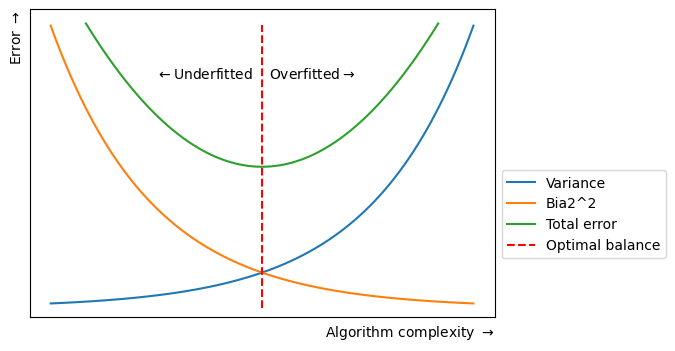
\includegraphics{section2_files/figure-pdf/cell-2-output-1.png}

}

\end{figure}

\begin{itemize}
\tightlist
\item
  \textbf{Correlation vs covariance:} correlation is a measure of
  relationship between two variables and says how strong are the
  variables related. Range is -1 to 1. Covariance represents the extent
  to which the variables change together in a cycle. This explains the
  systematic relationship between pair of variables where changes in one
  affect changes in another variable. Range is -inf to +inf, and is
  affected by scalability.
\item
  \textbf{Confounding variables} are extraneous variables in a
  statistical model that correlates directly or inversely with both the
  dependent and the independent variable. Left unchecked, confounding
  variables can introduce many research biases to your work, causing you
  to misinterpret your results.
\item
  \textbf{R-squared/coefficient of determination} is a statistical
  measure in a linear regression model that determines the proportion
  (percentage) of the variance in the dependent variable that can be
  explained by the independent variable. In other words, it evaluates
  the scatter of the data points around the fitted regression line,
  i.e.~shows how well the regression model explains observed data.
\end{itemize}

\[\begin{aligned}
R^{2} &= 1 - \frac{\text{Residual variance}}{\text{Total variance}} \\
&=\frac{\text{Total variance - Residual variance}}{\text{Total variance}} \\
&=\frac{\text{Explained variance}}{\text{Total variance}} \\
&=\text{Fraction of total variance explained}
\end{aligned}\]

\begin{itemize}
\item
  \textbf{p-value} is the measure of the statistical importance of an
  observation. We compute the p-value to understand whether the given
  data really describes the observed effect or not. If p\textless=0.05
  it suggests that there is only 5\% chance that the outcomes of an
  experiment are random and the null hypothesis must be rejected.
  \[ p_{value} = P(E|H_{0}) \]
\item
  \textbf{The statistical power} of a binary hypothesis test is the
  probability that the test rejects the null hypothesis when a specific
  alternative hypothesis is true
\item
  \textbf{Confidence interval} is a range of values likely containing
  the population parameter. \textbf{Confidence level} is denoted by
  1-\(\alpha\), where \(\alpha\) is level of significance (usually 5\%).
  \textbf{Point estimate} is an estimate of the population parameter
  (can be derived with Maximum Likelihood estimator for egz.)
  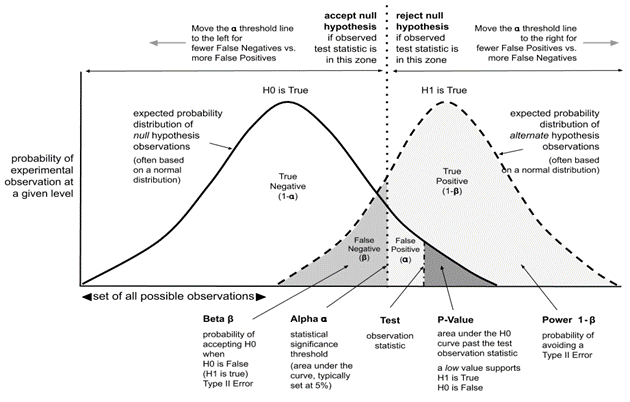
\includegraphics{Picture7.png}
\item
  \textbf{Univariate, bivariate and multivariate analysis:} univariate
  analysis allows us to understand the data and extract patterns and
  trends out of it. Bivariate analysis allows us to figure out the
  relationship between the variables. Multivariate analysis allows us to
  figure out the effects of all other variables (input variables) on a
  single variable (the output variable).
\item
  \textbf{Sampling} is the selection of individual members or a subset
  of the population to estimate the characters of the whole population.
  It is useful with datasets that are too large to efficiently analyze
  in full. There are two types of sampling techniques: probability and
  non-probability. \textbf{Resampling} is the process of
  changing/exchanging data samples, identifying the impact of these
  changes on model and prediction characteristics, and continuing until
  optimal results are achieved. It is done in cases of estimating the
  accuracy of sample statistics or validating models by using random
  subsets to ensure variations are handled (egz. Bootstraping,
  cross-validation)

  Types of biases that can occur during sampling: selection bias,
  undercoverage bias and survivorship bias. \textbf{Selection bias}
  occurs when a sample selection does not accurately reflect the target
  population. \textbf{Survivorship bias} is the logical error of
  focusing on aspects that support surviving a process and casually
  overlooking those that did not. This can lead to wrong conclusions in
  numerous ways.
\item
  \textbf{Bootstrap method} is a resampling method by independently
  sampling with replacement from an existing sample data with same
  sample size n, and performing inference among these resampled data.
\item
  \textbf{Normalization/Min-Max scaling} is used to transform features
  to be on a similar scale ({[}0,1{]} or {[}-1,1{]}). It is useful when
  there are no outliers.
  \[ X_{new} = (X - X_{min}) / (X_{max} - X_{min}) \] Normalization is
  useful when your data have different dimensions and the method you're
  employing doesn't make assumptions about the distirbution of you data.
\item
  \textbf{Standardization/Z-score} normalization is the transformation
  of features by subtracting from mean and dividing by standard
  deviation. It is not affected with outliers since its not bounded to a
  certain range. Changing the range of your data with scaling is
  different from changing the distribution of your data with
  Normalization. Also, standardization presupposes that the distribution
  of your data is Gaussian. \[ z = \frac{x-\mu}{\sigma}, \] where
  \(\mu\) represents the mean and \(\sigma\) represents the standard
  deviation.
\item
  \textbf{The Central limit theorem} says that, given a large enough
  sample size, the distirbution of sample averages/means will be
  approximtely normal. This means that we can use normal distirbution to
  make predictions about populations based on samples.
\item
  \textbf{The Law of large numbers} is a theorem that describes the
  result of performing the same experiment very frequently. It states
  that the sample mean, sample variance, and sample standard deviation
  converge to what they are trying to estimate
\item
  \textbf{Gradient}, for purposes of this paper, measures how much the
  output of a function changes if you change the inputs a little bit
  (from a given point).
\item
  \textbf{Categorical, continuous and ordinal variables.} An ordinal
  variable is a categorical variable for which the possible values are
  ordered.
\item
  \textbf{Histrograms vs boxplots:} Boxplots are more often used in
  comparing several datasets and take less space than histograms.
  Histograms are used to know and understand the probability
  distribution underlying a dataset
\item
  \textbf{Histograms vs bar graphs:} a bar graph is the graphical
  representation of categorical data, whereas a histogram is the
  graphical representation of data where data is grouped into continuous
  number ranges
\item
  \textbf{Kernel density estimation (KDE)} is a method for visualizing
  the distirbution of observations in dataset over a continuous interval
  or time period
\item
  \textbf{Histograms vs density plots:} an advantage that density plots
  have over histograms is that they're better at determining the
  distribution shape because they are not affected by the number of bins
  used.
\item
  \textbf{Akaike information Criterion (AIC):} is a mathematical method
  for evaluating how well a model fits the data it was generated from.
  In statistics, it is used to compare different possible models (model
  selection). Lower AIC scores are better!
\end{itemize}

\hypertarget{time-series-analysis}{%
\subsection{Time series analysis}\label{time-series-analysis}}

Time series analysis (TSA) is a mathematical approach for predicting or
forecasting the future pattern of data using historical data arranged in
a successive order for a particular time period. \emph{statsmodels.tsa}
package contains model classes and functions that are useful for time
series analysis.

\begin{itemize}
\item
  \textbf{Prediction vs forecasting:} prediction is concerned with
  estimating the outcomes of unseen data. Forecasting is a
  sub-discipline of prediction in which we are making predictions about
  the future on the basis of time series data, so the only difference is
  that we consider the temporal dimension
\item
  \textbf{Trend vs season vs cyclic:} A trend exists when there is a
  long-term increase or decrease in the data. It does not have to be
  linear. A seasonal pattern occurs when a time series is affected by
  seasonal factors such as the time of the year or the day of the week.
  Seasonality is always of a fixed and known frequency. A cycle occurs
  when the data exhibit rises and falls that are not of a fixed
  frequency.
\item
  \textbf{Rolling average/ moving average} is a metric that calculates
  trends over short periods of time using a set of data. Is uses smaller
  parts of the data and then rolls or moves for each new period.
  Calculating next rolling period involves leaving off your earliest
  unit and adding in your next unit. For egz., if you want to track down
  monthly data, take 12-months rolling period. After calculating average
  of 12 months, leave first month and add new month, then calculate
  average again for new rolling period. In that way, rolling period
  keeps moving.
\item
  \textbf{Augmented Dickey-Fuller test:} tests the null hypothesis that
  a unit root is present in a time series sample. It is a negative
  number, and the more negative it is, the stronger the rejection of the
  hypothesis that there is a unit root at some level of confidence.

  There are 3 main versions of the test (Dickey-Fuller test is presented
  for simplicity):

  \begin{enumerate}
  \def\labelenumi{\arabic{enumi}.}
  \tightlist
  \item
    Test for a unit root:
    \(\Delta y_{t} = \delta y_{t-1} + u_{t} \quad(u_{t} \text{ is error term})\)
  \item
    Test for a unit root with constant:
    \(\Delta y_{t} = a_{0} + \delta y_{t-1} + u_{t}\)
  \item
    Test for a unit root with constant and deterministic time trend:
    \(\Delta y_{t} = a_{0} + a_{1}t + \delta y_{t-1} + u_{t}\)
  \end{enumerate}

  -\textgreater{} Hypothesis: H0: δ = 0 (process is not stationary) H1:
  δ \textless{} 0 (process is stationary)

  -\textgreater{} from statsmodels.tsa.stattools import adfuller. For
  additional parameters, it is the best practice to put autolag=`AIC'.
  regression parameter has 4 parameters: `c' for only constant
  (default), `ct' for constant and trend, `ctt' for constant and linear
  and quadratic trend, `n' for no constant and no trend.

  -\textgreater{} Which version of test to choose? δ needs to be
  \textless= 0, so one way to find out is to see if it fits in the right
  interval. Other way is to compare AIC values and choose lowest. Also
  by inspecting data we can assume which to choose, but the best way is
  to perform all 3 types and inspect results.
\item
  \textbf{Stationary time series:} the only assumption in TSA is that
  the data is \emph{stationary}. Data is stationary when the variance
  and mean of the series are constant with time, with no periodic
  component (independent of time influence).

  \begin{itemize}
  \tightlist
  \item
    Check it with Augmented Dickey-Fuller test
  \item
    Trend can result in a varying mean over time, wheras seasonality can
    result in a changing variance over time, both which define a time
    series as being non-stationary. (stationary datasets are much easier
    to model).
  \item
    \textbf{Differencing} is a widely used data transform for making
    time series data stationary. Notice that some temporal structures
    may still exist after performing a differencing operation, such as
    in the case of a nonlinear trend. The number of times that
    differencing is performed is called the difference order. DataFrame
    diff() function can be used.
  \end{itemize}
\item
  There are two popular types of non-stationary time series:

  \begin{enumerate}
  \def\labelenumi{\alph{enumi}.}
  \tightlist
  \item
    \textbf{Trend-stationarity time series} are those whose mean trend
    is deterministic. In other words, the mean of the time series
    changes over time but at a constant rate. The time series is not
    stationary in the strict sense, but it is stationary in the sense
    that the trend is stable and predictable
  \item
    \textbf{Difference-stationarity time series} have a mean trend that
    is stochastic. In other words, the mean of the time series changes
    over time in a random pattern.
  \end{enumerate}
\item
  \textbf{Log transform:} time series with an exponential distribution
  can be made linear by taking the logarithm of the values. Log
  transforms are popular with time series data as they are effective at
  removing exponential variance
\item
  \textbf{Autocorrelation analysis} is used in detecting patterns and
  checking for randomness. The analysis involves looking at the
  Autocorrelation Function (ACF) and Partial Autocorrelation Function
  (PACF) plots.

  \begin{itemize}
  \tightlist
  \item
    Autocorrelation is a mathematical representation of the degree of
    similarity between a given time series and a lagged version of
    itself over successive time intervals. ACF function measures and
    plots the average correlation between data points in time series and
    previous values of the series measured for different lag lenghts.
  \item
    Partial autocorrelation is similar to autocorrelation except that
    each partial correlation controls for any correlation between
    observations of a shorter lag length. For egz., at second lag, the
    PACF measures the correlation between data points at time „t`` with
    data points at time „t-2``, while the ACF measures the same
    correlation but after controlling for the correlation between data
    points at time „t`` with those at time „t-1``.
  \item
    \emph{from statsmodels.graphics.tsaplots import plot\_acf,
    plot\_pacf}
  \item
    Stationarity of time series can be inspected with ACF plot (along
    with ADF test). In case the autocorrelations are positive for
    multiple lags, the series requires further differencing; but if lag
    1 autocorrelated itself pretty negatively, then the series is
    possibly over-differenced
  \end{itemize}
\end{itemize}

\hypertarget{models}{%
\subsubsection{Models}\label{models}}

\begin{itemize}
\item
  \textbf{AutoRegressive model (AR):} it is a linear model where current
  period values are a sum of past outcomes multiplied by a numeric
  factor. We denote it as AR(p), where „p`` is called the order of the
  model and represents the number of lagged values we want to include. p
  can be determined from PACF plot. For p=1:
  \[ X_{t} = C + \phi_{1}X_{t-1} + \varepsilon_{t}, \] The coefficient
  \(\phi_{1}\) is a numeric constant with value between -1 and 1. When
  multiplied with past value it represents a part which remains in the
  future. You would choose an AR model if you believe that previous
  observations have a direct effect on the time series.
\item
  \textbf{Moving Average (MA):} it's a statistic that captures the
  average change in data series over time. We denote it as MA(q), where
  „q`` is called the order of the model and represents the number of
  past forecast errors (or the size of the moving average window). q can
  be determined from ACF plot. You would choose an MA model if you
  believe that the errors have a direct effect on the time series.
\item
  \textbf{AutoRegressive Moving Average (ARMA):} p,q
\item
  \textbf{AutoRegressive Integrated Moving Average (ARIMA):} p,d,q..
  where d is the difference order
\item
  \textbf{AutoRegressive Moving Average with eXogeneous factors
  (ARMAX):} exogeneous variables are external data used in forecast
  (external effects)
\item
  \textbf{Seasonal AutoRegressive Integrated Moving Average (SARIMA):}
  p,d,q,P,D,Q,m.. where m is the number of time steps for a single
  seasonal period, p,d,q are trend elements and P,D,Q are seasonal
  elements
\item
  \textbf{Seasonal AutoRegressive Integrated Moving Average with
  eXogeneous factors (SARIMAX)}

  STEPS FOR BUILDING ONE OF THESE MODELS:

  \begin{enumerate}
  \def\labelenumi{\arabic{enumi})}
  \item
    Check for stationarity of time series and perform differencing if
    needed. This is because the term „autoregressive`` implies Linear
    Regression model (using its lags as predictors) and it works well
    for independent and non-correlated predictors
  \item
    Determine parameters. It can be done with inspecting acf/pacf plots
  \item
    Fit the model. Inspect coefficients and
    P(\textgreater\textbar z\textbar) with .summary() function and
    decide if it is needed for further tuning of parameters
  \item
    Check residuals for making sure model has captured adequte
    information from the data (they should look like white noise). If
    density looks normally distirbuted, model is ready.
  \item
    Make predictions (using .forecast() or .predict() function)
  \item
    Evaluate model predictions using common metrics (MAE, RMSE,..)

    \begin{itemize}
    \tightlist
    \item
      Alternatively, use \emph{pmdarima} package and \emph{auto\_arima}
      function to automate steps 1 to 3. Be aware that sometimes the
      manually fitted model is closer to the actual test set
    \item
      Alternatively, use plot\_diagnostics to automate step 4. Values of
      good fit:

      \begin{enumerate}
      \def\labelenumii{\alph{enumii}.}
      \tightlist
      \item
        Standardized residual: there are no obvious patterns in
        residuals, with values having a mean of zero
      \item
        The KDE curve should be very similar to the normal distribution
      \item
        Normal Q-Q: most of the data points should lie on the straight
        line
      \item
        Correlogram: 95\% of correlations for lag greater than zero
        should not be significant
      \end{enumerate}
    \item
      Suggestion: conduct time series cross-validation to select the
      best model, i.e.~repeat model assessment for different train /
      test sets
    \item
      Pro tip: if data shows exponential trend you can do a log
      transform before applying a model, then later apply inverse
      transformation (exponential function)
    \end{itemize}
  \end{enumerate}
\end{itemize}

\hypertarget{useful-tipsfunctions}{%
\paragraph{Useful tips/functions}\label{useful-tipsfunctions}}

\begin{itemize}
\tightlist
\item
  Date increment used for a date range:
  \emph{pandas.tseries.offsets.DateOffset}
\end{itemize}

\hypertarget{machine-learning}{%
\section{Machine learning}\label{machine-learning}}

Hypothesis in the content of ML represents a mathematical function that
an algorithm uses to represent the relationship between the target
variable and features. Learnings can be divided into supervised and
unsupervised learning.

\begin{longtable}[]{@{}
  >{\centering\arraybackslash}p{(\columnwidth - 2\tabcolsep) * \real{0.5000}}
  >{\centering\arraybackslash}p{(\columnwidth - 2\tabcolsep) * \real{0.5000}}@{}}
\toprule\noalign{}
\begin{minipage}[b]{\linewidth}\centering
\textbf{Supervised learning}
\end{minipage} & \begin{minipage}[b]{\linewidth}\centering
\textbf{Unsupervised learning}
\end{minipage} \\
\midrule\noalign{}
\endhead
\bottomrule\noalign{}
\endlastfoot
Works on the data that contains both inputs and the expected output,
i.e.~the labeled data & Works on the data that contains no mappings from
input to output, i.e.~the unlabeled data \\
Used to create models that can be employed to predict or classify things
& Used to extract meaningful information out of large volumes of data \\
Egz. Decision trees, logistic regression, svm & Egz. K-means clustering,
hierarchical clustering, apriori algorithm \\
\end{longtable}

\begin{itemize}
\tightlist
\item
  \textbf{Test set vs validation set:} test set is used to evaluate the
  performance of the trained model, and the validation set is part of
  the training set that is used to select parameters for avoiding model
  overfitting. (80\% training, 10\% validation, 10\% test)
\end{itemize}

\hypertarget{regression-and-classification-algorithms}{%
\subsection{Regression and classification
algorithms}\label{regression-and-classification-algorithms}}

\begin{itemize}
\item
  \textbf{Regression:} linear (when variables are continuous and
  numeric) and logistic (when variables are continuous and categorical)

  \begin{itemize}
  \tightlist
  \item
    \textbf{Linear regression} is supervised learning algorithm, which
    helps in finding the linear relationship between two variables. It
    finds the smallest sum of squared residuals that is possible for the
    dataset.
  \end{itemize}
\item
  \textbf{Classification} refers to a predictive modeling process where
  a class label is predicted for a given example of input data. It helps
  categorize the provided input into a label that other observations
  with similar features have.

  \begin{itemize}
  \item
    \textbf{Naive Bayes} is supervised classification ML algorithm based
    on the Bayes theorem, which deals with the probability of an event
    occuring given that another event has already occured
    (i.e.~mathematical formula for determining conditional probability).
    It is based on two assumptions, first, each feature/attribute
    present in the dataset is independent of another, and second, each
    feature carries equal importance. It has „naive`` in it because it
    assumes that the occurence of a certain feature is independent of
    the occurence of other features (hence each feature individually
    contributes to identify the result), which is unrealistic for
    real-world data
  \item
    \textbf{Support vector machine (SVM)} is a supervised ML model that
    considers the classification algorithms for two-group classification
    problems. It is a representation of the training data as points in
    space that are seperated into categories with the help of a clear
    gap that should be as wide as possible. \textbf{Kernel function} is
    used to transform the data that is not linearly separable into one
    that is. It is generalized dot product function used for the
    computing dot product of vectors xx and yy in high dimensional
    feature space. This transformation is based on kernel trick
    (projecting data onto a higher dimension space where it can be
    linearly divided by a plane).
  \item
    \textbf{Logistic regression} is classification algorithm that is
    used to predict the probability of certain classes based on some
    dependent variables. Estimating probability is done by using its
    underlying logistic function (sigmoid). In short, the logistic
    regression model computes a sum of the input features and calculates
    the logistic of the result.

    Altough it is classiciation algorithm (it predicts a discrete
    class), it is part of the regression family as it involves
    predicting outcomes based on quantitative relationships between
    variables. Unlike, linear regression, it accepts both continuous and
    discrete variables as input and its output is qualitative.

    Sigmoid function:
    \(\quad S(x) = \frac{1}{1 + e^{-x}} = \frac{e^{x}}{e^{x} + 1} = 1 - S(-x).\)
  \end{itemize}
\item
  \textbf{Elbow method} is used to select „k`` for k-means clustering.
  It plots the value of the cost function produced by different values
  of k (for egz. 1 to 15). k-means cost function is sum of squared
  distances of each data point to respective centroid of cluster to
  which the data points belong.
\item
  \textbf{A ROC curve} is a graph showing the performance of a
  classification model at all classification thresholds ({[}0,1{]}). It
  plots two parameters: true positive rate (sensitivity) and false
  positive rate (1-specificity). Also, decreasing the threshold moves up
  along the curve. Classifiers that give curves closer to the top-left
  corner indicate a better performance. Note that the ROC does not
  depend on the class distribution and this makes it useful for
  evaluating classifiers predicting rare events such as diseases or
  disasters. In contrast, evaluating performance using accuracy would
  favor classifiers that always predict a negative outcome for rare
  events. To compare different classifiers, it is useful to summarize
  the performance of each classifier into a single measure- \textbf{AUC}
  (area under the ROC curve). The AUC is the probability the model will
  score a randomly chosen positive class higher than a randomly chosen
  negative class.
\item
  CART is name for classification and regression trees
\item
  \textbf{Decision tree} is non-parametric model that can be used for
  both classification and regression. Non-parametric means that they
  don't increase their number of parameters as we add more features.
  They are constructed using nodes and branches, where the root node
  testes a feature which best splits the data. Decision trees are built
  by recursively splitting our training samples using the features from
  the data that work best for the specific task. The process is done by
  evaluating certain metrics („information entropy``), depending if the
  feature is dicrete or continuous.

  Steps are:

  \begin{enumerate}
  \def\labelenumi{\arabic{enumi}.}
  \tightlist
  \item
    Take the entire data set as input
  \item
    Look for a split that maximizes the separation of the classes
  \item
    Apply the split (divide step)
  \item
    Re-apply steps 1) and 2) to the divided data
  \item
    Stop when you meet stopping criteria
  \item
    Pruning (clean up the tree if you went too far)
  \end{enumerate}

  \textbf{Entropy} in ML is the measurement of disorder or impurities in
  the information processed.

  \[ E = -\sum^{N}_{i=1}P_{i}\text{log}_{2}P_{i}, \] where \(P_{i}\) is
  probability of randomly selecting an example in class i.

  \textbf{Information gain} is a measure of how much entropy is reduced
  when a particular feature is used to split the data. It calculates the
  difference between entropy before and after the split.

  \textbf{Pruning} is a technique that simplifies the decision tree by
  reducing the rules. It helps to avoid the complexity and improves
  accuracy.
\item
  \textbf{Random forest} is a model built up of a number of decision
  trees. If you split the data into different packages and make a
  decision tree in each of the different groups of data. The random
  forest brings all those trees together (individual trees need to have
  low correlations with each other).

  Steps to build a model:

  \begin{enumerate}
  \def\labelenumi{\arabic{enumi}.}
  \tightlist
  \item
    Randomly select \emph{k} features from a total of \emph{m} features
    (k\textless\textless m)
  \item
    Among the \emph{k} features, calculate the node using the best split
    point
  \item
    Split the node into daughter nodes using the best split
  \item
    Repeat steps two and three until leaf nodes are finalized
  \item
    Build forest by repeating steps one to four for \emph{n} times to
    create \emph{n} number of trees
  \end{enumerate}
\end{itemize}

\hypertarget{tuning-model-parameters-evaluation}{%
\subsection{Tuning model parameters,
evaluation}\label{tuning-model-parameters-evaluation}}

\textbf{Overfitting} referes to a model that is only set for a very
small amount of data and ignores the bigger picture.

There are three main methods to avoid it:\\
\hspace*{0.333em}\hspace*{0.333em}- feature selection\\
\hspace*{0.333em}\hspace*{0.333em}- cross-validation\\
\hspace*{0.333em}\hspace*{0.333em}- feature engineering (creating more
data samples using the existing set of data, for egz. In CNN it is
producing new images by rotating, scaling, flipping,..)\\
\hspace*{0.333em}\hspace*{0.333em}- regularization\\
\hspace*{0.333em}\hspace*{0.333em}- early stopping (regularization
technique that identifies the point from where the training data leads
to generalization error\\
\hspace*{0.333em}\hspace*{0.333em}- dropouts (regularization technique
used in the case of NN where we randomly deactivate a proportion of
neurons in each layer)

\begin{itemize}
\tightlist
\item
  Dimensionality reduction helps in compressing data and removing
  redundant features. \textbf{Feature selection} is the method of
  reducing the input variable to your model by using only relevant data
  and getting rid of noise in data.
\end{itemize}

\hypertarget{feature-selection}{}
\begin{figure}[H]

{\centering \includegraphics[width=4in,height=2in]{section2_files/figure-latex/dot-figure-2.png}

}

\end{figure}

\hfill\break
\(~~~~~~~~\)- Filter method: features are dropped based on their
relation to the output, or how they are correlating to the output

\(~~~~~~~~\)- Wrapper method: we split our data into subsets and train a
model using this. Based on the output of the model, we add and subtract
features and train the model again. It forms the subsets using a greedy
approach and evaluates the accuracy of all the possible combinations of
features.

\begin{itemize}
\item
  \textbf{Multicollinearity} is reflected in the model when independent
  variables in a multiple regression model are deduced to possess high
  correlations with each other. It can be overcomed by removing a few
  highly correlated variables from the equation.
\item
  \textbf{Feature scaling} is one of the most important data
  preprocessing steps in ML. Algorithms that compute the distance
  between the features are biased towards numerically larger values if
  the data is not scaled. Most popular are normalizaton and
  standardization. Also, sklearn library provides transformers
  \emph{MinMaxScaler} and \emph{StandardScaler}.
\item
  \textbf{Feature engineering} is the method that is used to create new
  features from the given dataset using the existing variables. For egz.
  Imputation, discretization, categorical encoding,..
\item
  \textbf{Cross-validation} is a statistical method used to estimate the
  performance of ML models. It is used to protect against overfitting in
  a predictive model, particularly in a case where the amount of data
  may be limited.

  \textbf{k-fold cross validation} guarantees that the score of our
  model does not depend on the way we picked the train and test set. The
  data is first randomly divided into k number of subsets. For each
  subset in your dataset, build your model on k-1 subsets of the
  dataset. Then, test the model to check the efectiveness for kth
  subset. Repeat this until each of k-subsets has served as the test
  set. The average of your \emph{k} recorded accuracy is called the
  cross-validation accuracy and will serve you as your performance
  metric for the model. The disadvantage of this method is that the
  training algorithm has to be rerun from scratch \emph{k} times. Also,
  it only estimates the accuracy but does not improve it.
\item
  \textbf{Regularization} is a form of regression which discourages
  learning a more complex or flexible model, so as to avoid the risk of
  overfitting. The general idea is to penalize complicated models by
  adding an additional penalty to the loss function in order to generate
  a larger loss. In this way, we can discourage the model from learning
  too many details and the model is much more general. Three popular
  methods are Ridge regression (L2 norm, most used), Lasso (L1 norm) and
  Dropout (used in neural networks). If there is noise in the training
  data, then estimated coefficients won't generalize well to the future
  data and this is where regularization comes in. It happens by adding a
  tuning parameter λ that decides how much we want to penalize the
  flexibility of our model. As the value of λ rises, it reduces the
  value of coefficients and thus reducing the variance. Till a point,
  this increase in λ is beneficial as it is only reducing the variance
  (hence avoiding overfitting), without loosing any important properties
  in the data. But after certain value, the model starts lossing
  important properties, giving rise to bias in the model and thus
  underfitting.
\item
  \textbf{Ensemble learning} is combining several individual models
  together to improve performance.

  \begin{enumerate}
  \def\labelenumi{\arabic{enumi}.}
  \tightlist
  \item
    \textbf{Boosting} is one of the ensemble learning methods where we
    create multiple models and sequentially train them by combining weak
    models iteratively in a way that training a new model depends on the
    models trained before it. We take the patterns learned by a previous
    model and test them on a dataset when training the new model. In
    each iteration, we give more importance to observations in the
    dataset that are incorrectly handled or predicted by previous
    models. It is useful in reducing bias also.
  \item
    \textbf{Bagging} is an ensemble learning method where we generate
    some data using the bootstrap method, in which we use an already
    existing dataset and generate multiple samples of the „N`` size.
    This bootstrapped data is then used to train multiple models in
    parallel, which makes it more robust than a simple model. Once all
    the models are trained and it is time to make a prediction, we make
    predictions using all the trained models and then average the result
    in the case of regression, and for classification, we choose the
    result that has the highest frequency.
  \item
    \textbf{Stacking} is an ensemble learning method where we can
    combine weak models that can additionaly use different learning
    algorithms as well. These learners are called heterogeneous learners
    (boosting and bagging are homogeneous learners). Stacking works by
    training multiple and different weak models or learners and then
    using them together by training another model, called a meta-model,
    to make predictions.
  \end{enumerate}
\end{itemize}

Three commonly used methods for finding the sweet spot between simple
and complicated models are: regularization, boosting and bagging.

\begin{itemize}
\tightlist
\item
  \textbf{Gradient descent,} in ML, is an iterative method that
  minimizes the cost function parametrized by model parameters. This
  improves the learning model's efficacy by providing feedback to the
  model so that it can adjust the parameters to minimize the error and
  find the local or global minimum. Gradient measures the change in
  parameter with respect to the change in error. \textbf{Learning rate}
  or step size is the size of the steps that are taken to reach the
  minimum. This is typically a small value, and it is evaluated and
  updated based on the behavior of the cost function. High learning
  rates result in larger steps but risks overshooting the minimum. There
  are 3 types of gradient descent method:

  \begin{itemize}
  \tightlist
  \item
    \textbf{batch gradient descent:} computation is carried out on the
    entire dataset
  \item
    \textbf{stochastic gradient descent:} computation is carried over
    only one training sample
  \item
    \textbf{mini batch gradient descent:} a small number/batch of
    training samples is used for computation
  \end{itemize}
\end{itemize}

\hypertarget{deep-learning}{%
\section{Deep learning}\label{deep-learning}}

Deep learning is an advanced version of neural networks (NNs with more
than three layers) to make the machines learn from data.

\begin{itemize}
\tightlist
\item
  \textbf{RNN} (reccurent neural network) is an algorithm that uses
  sequential data (i.e.~data that are ordered into sequences) such as
  timeseries, stock market, temperature, etc.
\item
  \textbf{NLP} (natural language processing) deals with the study of how
  computers learn a massive amount of textual data through programming
\item
  \textbf{Batch normalization} is a technique for training very deep
  neural networks that standardize the inputs to a layer for each
  mini-batch. This has the effect of stabilizing the learning process
  and dramatically reducing the number of training epochs required to
  train deep networks. After this, model is less sensitive to
  hyperparameter tuning, high learning rates become acceptable (which
  results in faster training of the model), weight initialization
  becomes an easy task,..
\item
  A perceptron** is the simplest NN that contains a single neuron that
  performs 2 functions. The first function is to perform the weighted
  sum of all the inputs and the second is an activation function
\item
  \textbf{Autoencoders} are learning networks which transform inputs
  into outputs with minimum possible errors. Can be used in anomaly
  detection.
\end{itemize}

\bookmarksetup{startatroot}

\hypertarget{summary}{%
\chapter{Summary}\label{summary}}

In summary, this book has no content whatsoever.

\bookmarksetup{startatroot}

\hypertarget{references}{%
\chapter*{References}\label{references}}
\addcontentsline{toc}{chapter}{References}

\markboth{References}{References}

\hypertarget{refs}{}
\begin{CSLReferences}{1}{0}
\leavevmode\vadjust pre{\hypertarget{ref-knuth84}{}}%
Knuth, Donald E. 1984. {``Literate Programming.''} \emph{Comput. J.} 27
(2): 97--111. \url{https://doi.org/10.1093/comjnl/27.2.97}.

\end{CSLReferences}



\end{document}
